% =====================================================================
% TEMPLATE ELABORASI SATU KOMPONEN
% Salin file ini menjadi komponen_NAMA.tex, lalu ganti placeholder.
% Struktur ini diselaraskan secara generik mengikuti alur dht22.tex.
% Jangan meng-input file template ini secara langsung ke bab.
% =====================================================================

\subsection{HC-SR501 -- Sensor Gerak PIR}
\label{subsec:hc-sr501}

% ---------------------------------------------------------------------
\subsubsection{Identitas dan Fungsi}
\begin{wrapfigure}{r}{0.3\textwidth}% 'r' untuk posisi kanan, '0.25\textwidth' untuk lebar gambar
	\vspace{-20pt}
	\centering
	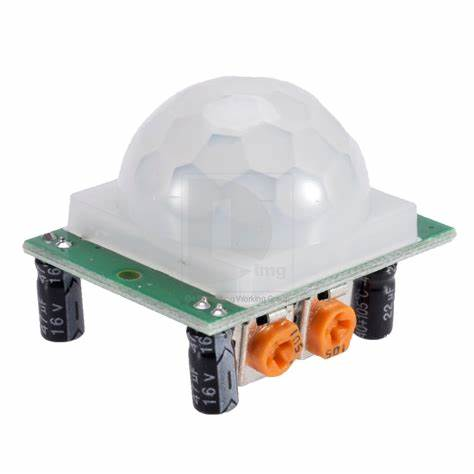
\includegraphics[width=\linewidth]{images/front_hc-sr501.jpg} % Ganti dengan nama file gambar Anda
	\caption{Sensor PIR HC-SR501.}
	\label{fig:hc-sr501_pir_sensor}
\end{wrapfigure}

Modul sensor gerak HC-SR501 merupakan sensor inframerah  pasif (\textit{Passive Infrared} / PIR) yang berfungsi untuk mendeteksi keberadaan atau pergerakan objek berbasis radiasi termal (inframerah) yang dipancarkan oleh tubuh manusia, hewan, atau benda bergerak lainnya. HC-SR501 dikategorikan sebagai \textbf{sensor digital} karena menghasilkan \textit{output} tingkat logika (\texttt{HIGH / LOW}) secara langsung. Modul ini memiliki konsumsi daya yang sangat rendah, antarmuka-antarmuka digital yang sangat sederhana tanpa memerlukan pustaka pemroses khusus, rentang sudut dan jarak deteksi yang luas, serta tersedianya potensiometer untuk penyesuaian sensitivitas dan \textit{delay} waktu secara fleksibel pada tingkat perangkat keras.

\begin{table}[H]
	\centering
	\caption{Identitas komponen HC-SR501}
	\label{tab:hc_sr501_identitas}
	\small
	\begin{tabularx}{\textwidth}{@{}lX@{}}
		\toprule
		Parameter          & Keterangan                                                     \\
		\midrule
		Nama komponen      & HC-SR501 Motion Detector Module                                \\
		Model/part number  & HC-SR501 (BISTOF / LHI778 / BISS0001)                          \\
		Jenis              & Sensor Digital Pasif (Passive Infrared Sensor)                 \\
		Fungsi utama       & Mendeteksi pergerakan objek berbasis radiasi inframerah termal \\
		Sumber dokumentasi & HC-SR501 PIR Motion Sensor Datasheet (ElectroniLab)  \\
		\bottomrule
	\end{tabularx}
\end{table}

% ---------------------------------------------------------------------
\subsubsection{Prinsip Kerja}
Sensor HC-SR501 bekerja berdasarkan prinsip \textbf{efek piroelektrik}, yaitu fenomena perubahan muatan listrik pada kristal piroelektrik ketika menerima variasi fluks radiasi inframerah ($IR$). Sensor ini tidak memancarkan radiasi sendiri , melainkan hanya menerima paparan energi panas alami dari objek dengan suhu di atas nol mutlak ($0\,\text{K}$). Uraian elemen-elemen penyusun internal modul adalah sebagai berikut:

\begin{enumerate}
	\item \textbf{Elemen Transduser Utama:}
	      Transduser primer berupa sensor piroelektrik dual-elemen (seperti LHI778 atau PIR28) yang dilapisi oleh lensa Fresnel. Lensa Fresnel berfungsi memfokuskan radiasi inframerah dari berbagai sudut pandang (hingga $120^\circ$) serta membagi area deteksi menjadi beberapa zona sudut. Ketika objek hangat melintas di depan sensor, pancaran radiasi inframerah memotong elemen pertama terlebih dahulu kemudian elemen kedua. Perbedaan diferensial radiasi yang diterima oleh kedua elemen piroelektrik memicu terjadinya fluktuasi muatan listrik ($\Delta V$).

	      \begin{figure}[htbp]
		      \centering
		      \begin{subfigure}[b]{0.4\textwidth}
			      \centering
			      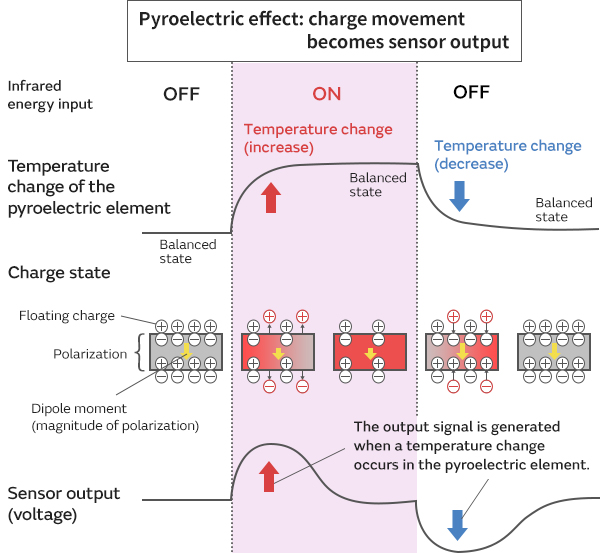
\includegraphics[width=\textwidth]{images/piroelektrik_effect.jpg}
			      %\fbox{\parbox[c][3.5cm][c]{\textwidth}{\centering Image 1 / Diagram A}}
			      \caption{Diagram efek piroelektrik.}
			      \label{fig:piroelektrik_effect}
		      \end{subfigure}
		      \hfill % Adds horizontal space between the two minipages
		      \begin{subfigure}[b]{0.48\textwidth}
			      \centering
			      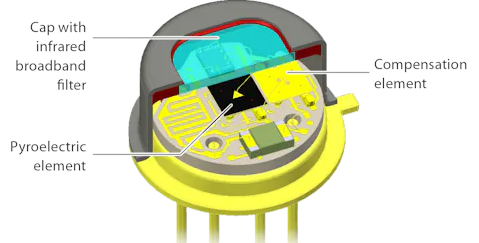
\includegraphics[width=\textwidth]{images/internal_pir.png}
			      % \fbox{\parbox[c][3.5cm][c]{\textwidth}{\centering Image 2 / Lensa Fresnel}}
			      \caption{Internal sensor PIR.}
			      \label{fig:fresnel_lens}
		      \end{subfigure}
		      \caption{Prinsip kerja dan diagram internal elemen sensoris pada HC-SR501.}
		      \label{fig:hc_sr501_gabungan}
	      \end{figure}


	\item \textbf{Elemen Pengkondisi Sinyal / Sirkuit Internal:}
	      Sinyal mikrovolt yang dihasilkan oleh elemen piroelektrik diproses oleh IC pengkondisi sinyal khusus \textbf{BISS0001} (\textit{Micro Power PIR Motion Detector IC}). Sirkuit internal ini terdiri dari dua tahap tahap penguat sinyal, \textit{Band-Pass Filter} untuk membuang \textit{noise} frekuensi lingkungan, serta \textit{window comparator} untuk mengubah tegangan analog diferensial menjadi sinyal digital TTL pada pin OUT.
\end{enumerate}

\begin{figure}[htbp]
	\centering
	% Ganti dengan file skematik rangkaian aktual atau tangkapan layar simulasi Wokwi
	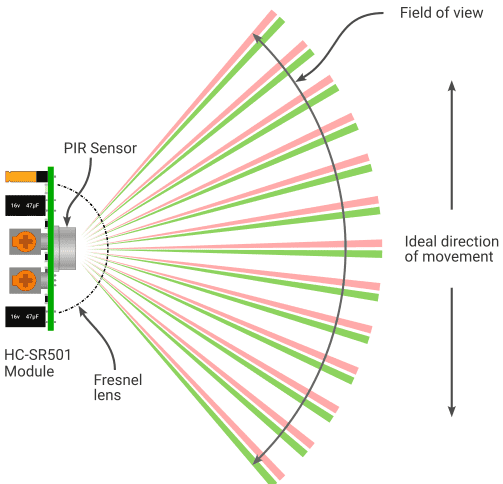
\includegraphics[width=0.50\textwidth]{images/hc-sr501_pov.png}
	%\fbox{\parbox[c][5cm][c]{0.70\textwidth}{\centering Tempatkan tangkapan layar simulasi Wokwi atau diagram skematik di sini}}
	\caption{Sudut deteksi dan arah pergerakan optimal sensor PIR HC-SR501.}
	\label{fig:hc-sr501-sensoris-range}
\end{figure}


\paragraph{Konsep dan Formulasi Matematis Terkait}
Besarnya radiasi termal yang dipancarkan oleh objek dan ditangkap oleh sensor mengikuti Hukum Stefan-Boltzmann:

\begin{equation}
	P = \varepsilon \cdot \sigma \cdot A \cdot (T^4 - T_0^4)
	\label{eq:hc_sr501_formulasi}
\end{equation}

\noindent di mana:
\begin{itemize}
	\item $P$ = Daya radiasi inframerah yang diterima oleh sensor ($\text{W}$).
	\item $\varepsilon$ = Emisivitas permukaan objek ($0 \le \varepsilon \le 1$, tubuh manusia $\approx 0{,}98$).
	\item $\sigma$ = Konstanta Stefan-Boltzmann ($5{,}67 \times 10^{-8}\,\text{W/m}^2\text{K}^4$).
	\item $A$ = Luas area pemancar inframerah yang terdeteksi ($\text{m}^2$).
	\item $T$ = Suhu mutlak permukaan objek ($\text{K}$).
	\item $T_0$ = Suhu mutlak lingkungan sekitar ($\text{K}$).
\end{itemize}

Sirkuit BISS0001 akan menghasilkan logika HIGH pada output apabila perubahan tegangan diferensial akibat variasi daya radiasi ($\Delta P$) melampaui batas sensitivitas yang diatur melalui potensiometer $V_{TH}$.

% ---------------------------------------------------------------------
\subsubsection{Alur Kerja Internal dan Protokol Komunikasi}
Alur pemrosesan data pada modul HC-SR501 mengikuti pola \textbf{Input $\rightarrow$ Proses $\rightarrow$ Output}:
\begin{enumerate}
	\item \textbf{Input:} Perubahan fluks inframerah akibat pergerakan objek bermassa panas yang melewati zona deteksi lensa Fresnel.
	\item \textbf{Proses:} Pemrosesan sinyal oleh IC BISS0001 yang meliputi penguatan sinyal diferensial AC, pemfilteran frekuensi gerakan manusia ($0{,}1\text{ s.d. }10\,\text{Hz}$), penentuan \textit{delay time} melalui jaringan sirkuit $RC$, serta evaluasi mode \textit{trigger} (\textit{repeatable} / \textit{non-repeatable} melalui \textit{jumper}).
	\item \textbf{Output:} Pulsa logika digital $3{,}3\,\text{V}$ (HIGH) saat pergerakan terdeteksi, atau $0\,\text{V}$ (LOW) saat kondisi \textit{idle} (tidak ada pergerakan).
\end{enumerate}

\paragraph{Detail Sinyal Komunikasi}
Modul HC-SR501 tidak menggunakan protokol transmisi berbasis paket byte (seperti I$^2$C, SPI, atau UART), melainkan memancarkan sinyal logika diskret biner (\textit{Discrete Digital Output}) yang dikendalikan secara langsung oleh IC pengkondisi BISS0001. Siklus tanggapan sinyal terhadap peristiwa pergerakan fisik (\textit{movement event}) terbagi menjadi empat fase utama:

\begin{itemize}
    \item \textbf{Inisialisasi Keadaan Awal (\textit{Power-Up Warm-Up}):} Saat pertama kali diberi catu daya, modul memerlukan waktu persiapan selama $30\text{ s.d. }60\,\text{detik}$ untuk menstabilkan komparator internal dan pembanding ambang batas. Pada interval ini, sinyal keluaran $V_{\text{OUT}}$ dapat berfluktuasi secara acak sebelum memasuki kondisi siap (\textit{idle}).

    \item \textbf{Respons Peristiwa Pergerakan \& Latensi Deteksi ($t_{\text{lat}}$):} Ketika objek termal bergerak melintasi kisi Lensa Fresnel, perubahan fluks radiasi inframerah menghasilkan diferensial muatan piroelektrik. Terdapat jeda latensi tanggapan singkat $t_{\text{lat}}$ ($< 0{,}5\,\text{detik}$) bagi komparator IC BISS0001 untuk memvalidasi ambang sinyal sebelum memicu pin OUT beralih dari $0\,\text{V}$ (LOW) ke $3{,}3\,\text{V}$ (HIGH).

    \item \textbf{Format Transmisi \& Waktu Tunda ($T_x$):} Durasi logika HIGH pada pin OUT bertahan selama rentang waktu tunda $T_x$ ($0{,}5\text{ s.d. }200\,\text{detik}$) yang disesuaikan melalui potensiometer \textit{Time Delay}. Mekanisme perhitungan $T_x$ terhadap peristiwa pergerakan susulan dipengaruhi secara langsung oleh konfigurasi \textit{jumper}:
          \begin{itemize}
              \item \textbf{Mode L (\textit{Non-repeatable Trigger}):} Durasi $T_x$ dihitung secara mutlak mulai dari \textbf{awal terdeteksinya pemicuan} (\textit{rising edge} sinyal OUT). Sinyal OUT akan beralih kembali ke logika LOW tepat setelah durasi $T_x$ usai, meskipun pergerakan fisik objek masih terus berlangsung di dalam jangkauan deteksi sensor.
              \item \textbf{Mode H (\textit{Repeatable Trigger}):} Durasi $T_x$ dihitung mulai dari \textbf{saat akhir pergerakan fisik berhenti} (\textit{falling edge} dari peristiwa pergerakan). Selama pergerakan fisik terus terdeteksi, pewaktu internal IC BISS0001 direset secara berulang (\textit{continuous re-trigger}) sehingga sinyal OUT dipertahankan pada logika HIGH selama durasi total \textbf{Pergerakan Fisik $+ T_x$}.
          \end{itemize}

    \item \textbf{Masa Penguncian (\textit{Inhibit / Blocking Time} $T_i$):} Sesaat setelah sinyal OUT kembali ke logika LOW, IC BISS0001 menerapkan masa jeda internal $T_i$ sebesar $\approx 2{,}5\,\text{detik}$ (ditentukan oleh komponen internal $R_i$ dan $C_i$). Selama periode ini, sensor mengunci penerimaan sinyal diferensial sehingga pergerakan baru tidak akan memicu keluaran HIGH hingga masa $T_i$ berakhir.
\end{itemize}

\begin{figure}[htbp]
    \centering
    \begin{tikzpicture}[x=0.18mm, y=10mm, >=Stealth, font=\sffamily\small]

        % =================================================================
        % SUB-DIAGRAM 1: Mode L (Non-repeatable Trigger)
        % =================================================================
        \begin{scope}[shift={(0,0)}]
            \node[font=\bfseries\small, anchor=west] at (80, 3.2) {(a) Mode L (\textit{Non-repeatable Trigger})};

            % Axis
            \draw[->, color=gray!60, thick] (0, 0) -- (600, 0) node[right, color=black] {\textit{t}};
            \draw[->, color=gray!60, thick] (0, 0) -- (0, 2.8) node[above, color=black] {OUT};

            % Level Logika Sumbu Y
            \node[left, font=\scriptsize] at (0, 1.8) {\textbf{HIGH (3.3V)}};
            \node[left, font=\scriptsize] at (0, 0.4) {\textbf{LOW (0V)}};

            \draw[dotted, color=gray!40] (0, 1.8) -- (580, 1.8);
            \draw[dotted, color=gray!40] (0, 0.4) -- (580, 0.4);

            % Garis Putus-Putus Periode Pergerakan Fisik (x=40 ke x=220)
            \draw[thick, color=purple, dash pattern=on 3pt off 2pt] (40, 2.3) -- (220, 2.3);
            \draw[thick, color=purple, dash pattern=on 3pt off 2pt] (390, 2.3) -- (470, 2.3);
            \node[color=purple, font=\tiny, above] at (130, 2.3) {Periode Gerakan Fisik};
            \node[color=purple, font=\tiny, above] at (430, 2.3) {Gerakan 2};

            % Garis Vertikal Acuan Latensi
            \draw[dashed, color=purple!60] (40, 2.3) -- (40, 0.2);
            \draw[dashed, color=gray!60] (70, 1.8) -- (70, 0.2);

            % Sinyal OUT Mode L (Naik di x=70 setelah latensi t_lat dari x=40)
            \draw[ultra thick, color={rgb,255:red,30;green,64;blue,175}]
            (0, 0.4) -- (70, 0.4) -- (70, 1.8) -- (210, 1.8) -- (210, 0.4) -- (390, 0.4) -- (390, 1.8) -- (530, 1.8) -- (530, 0.4) -- (580, 0.4);

            % Anotasi Delay Latensi (t_lat)
            \draw[stealth-stealth, color=purple, thick] (40, 1.1) -- (70, 1.1)
            node[midway, above, font=\tiny] {$t_{\text{lat}}$};

            % Anotasi Delay Tx dihitung dari pemicuan sinyal (x=70 ke x=210)
            \draw[stealth-stealth, color={rgb,255:red,30;green,64;blue,175}] (70, 1.1) -- (210, 1.1)
            node[midway, below, font=\tiny] {\shortstack{$T_x$ dari\\Awal Pemicuan}};
            \draw[stealth-stealth, color={rgb,255:red,217;green,119;blue,6}] (210, -0.3) -- (290, -0.3) node[midway, below, font=\tiny] {Blocking $T_i \approx 2.5\text{s}$};
            \node[color=red!80!black, font=\tiny, align=left] at (290, 0.7) {Tetap LOW meskipun\\masih ada gerakan};
        \end{scope}

        % =================================================================
        % SUB-DIAGRAM 2: Mode H (Repeatable Trigger)
        % =================================================================
        \begin{scope}[shift={(0,-5.5)}]
            \node[font=\bfseries\small, anchor=west] at (80, 3.2) {(b) Mode H (\textit{Repeatable Trigger})};

            % Axis
            \draw[->, color=gray!60, thick] (0, 0) -- (600, 0) node[right, color=black] {\textit{t}};
            \draw[->, color=gray!60, thick] (0, 0) -- (0, 2.8) node[above, color=black] {OUT};

            % Level Logika Sumbu Y
            \node[left, font=\scriptsize] at (0, 1.8) {\textbf{HIGH (3.3V)}};
            \node[left, font=\scriptsize] at (0, 0.4) {\textbf{LOW (0V)}};

            \draw[dotted, color=gray!40] (0, 1.8) -- (580, 1.8);
            \draw[dotted, color=gray!40] (0, 0.4) -- (580, 0.4);

            % Garis Putus-Putus Periode Pergerakan Fisik (x=40 ke x=220)
            \draw[thick, color=purple, dash pattern=on 3pt off 2pt] (40, 2.3) -- (220, 2.3);
            \draw[thick, color=purple, dash pattern=on 3pt off 2pt] (440, 2.3) -- (480, 2.3);
            \node[color=purple, font=\tiny, above] at (130, 2.3) {Periode Gerakan Fisik};
            \node[color=purple, font=\tiny, above] at (460, 2.3) {Gerakan 2};

            % Garis Vertikal Acuan Latensi & Akhir Gerakan
            \draw[dashed, color=purple!60] (40, 2.3) -- (40, 0.2);
            \draw[dashed, color=gray!60] (70, 1.8) -- (70, 0.2);
            \draw[dashed, color=gray!60] (220, 2.3) -- (220, 0.8);

            % Sinyal OUT Mode H (Naik di x=70 setelah latensi t_lat dari x=40)
            \draw[ultra thick, color={rgb,255:red,15;green,118;blue,110}]
            (0, 0.4) -- (70, 0.4) -- (70, 1.8) -- (340, 1.8) -- (340, 0.4) -- (440, 0.4) -- (440, 1.8) -- (580, 1.8);

            % Anotasi Delay Latensi (t_lat)
            \draw[stealth-stealth, color=purple, thick] (40, 1.1) -- (70, 1.1)
            node[midway, above, font=\tiny] {$t_{\text{lat}}$};

            % Anotasi Durasi Selama Gerakan (x=70 ke x=220) & Anotasi Delay Tx dari Akhir Gerakan (x=220 ke x=340)
            \draw[stealth-stealth, color={rgb,255:red,15;green,118;blue,110}] (70, 1.1) -- (220, 1.1)
            node[midway, below, font=\tiny] {\shortstack{HIGH selama\\ada gerakan}};
            \draw[stealth-stealth, color={rgb,255:red,15;green,118;blue,110}] (220, 1.1) -- (340, 1.1)
            node[midway, below, font=\tiny] {\shortstack{$T_x$ dari\\Akhir Gerakan}};

            \draw[->, color=red!80!black, thick] (130, 1.7) -- (130, 1.3) node[midway, right, font=\tiny] {Reset $T_x$};
            \draw[->, color=red!80!black, thick] (190, 1.7) -- (190, 1.3) node[midway, right, font=\tiny] {Reset $T_x$};
            \draw[stealth-stealth, color={rgb,255:red,217;green,119;blue,6}] (340, -0.3) -- (420, -0.3) node[midway, below, font=\tiny] {Blocking $T_i$};
        \end{scope}

    \end{tikzpicture}
    \caption{Perbandingan mekanisme perhitungan waktu tunda $T_x$ dan latensi deteksi $t_{\text{lat}}$ pada Mode L (\textit{Non-repeatable}) dan Mode H (\textit{Repeatable}).}
    \label{fig:hc_sr501_timing_combined}
\end{figure}


% ---------------------------------------------------------------------
\subsubsection{Besaran yang Diukur atau Dikendalikan}
HC-SR501 mengukur perubahan kuantitas radiasi termal inframerah terfokus ($\Delta IR$) yang dikonversi menjadi sinyal ketersediaan objek bergerak biner di dalam jangkauan sudut deteksinya. Karakteristik besaran operasional modul ini dirangkum pada Tabel~\ref{tab:hc_sr501_karakteristik_besaran}.

\begin{table}[H]
    \centering
    \caption{Karakteristik besaran operasional modul HC-SR501}
    \label{tab:hc_sr501_karakteristik_besaran}
    \small
    \begin{tabularx}{\textwidth}{@{} p{3.8cm} >{\hsize=0.7\hsize}X >{\hsize=1.3\hsize}X @{}}
        \toprule
        Parameter & Nilai & Keterangan \\
        \midrule
        Besaran Utama & Perubahan Fluks Inframerah ($\Delta IR$) & Fluktuasi radiasi termal akibat pergerakan objek \\
        Rentang Kerja (Jarak) & $3\text{ s.d. }7\,\text{m}$ & Dapat diatur secara manual via potensiometer sensitivitas \\
        Sudut Deteksi & $< 120^\circ$ & Sudut kerucut efektif (\textit{effective cone angle}) Lensa Fresnel \\
        Resolusi & Biner ($0$ / $1$) & Deteksi logika (\textit{Boolean}): HIGH ($3{,}3\,\text{V}$) / LOW ($0\,\text{V}$) \\
        Akurasi / Sensitivitas & Optimal pada $\Delta T \ge 3^\circ\text{C}$ & Sensitif terhadap perbedaan suhu target dengan lingkungan \\
        Pengulangan (\textit{Repeatability}) & Berdasarkan konfigurasi \textit{jumper} & Mode H (\textit{Repeatable}) atau Mode L (\textit{Non-repeatable}) \\
        Waktu Respons (Latensi) & $< 0{,}5\,\text{s}$ & Latensi pemicuan dari munculnya gerakan hingga sinyal OUT beralih ke HIGH \\
        Durasi Blocking Sinyal ($T_i$) & $\approx 2{,}5\,\text{s}$ & Periode penguncian (\textit{blocking time}) internal BISS0001 saat gerakan baru diabaikan \\
        Durasi Sinyal Keluaran ($T_x$) & $0{,}5\text{ s.d. }200\,\text{s}$ & Lebar pulsa HIGH yang dapat disesuaikan secara manual via potensiometer $T_x$ \\
        \bottomrule
    \end{tabularx}
\end{table}
% ---------------------------------------------------------------------
\subsubsection{Karakteristik Sinyal}
Sinyal keluaran pada pin OUT modul HC-SR501 memiliki karakteristik listrik sebagai berikut:

\begin{equation}
	V_{\text{OUT}} =
	\begin{cases}
		3{,}3\,\text{V} \, (\text{HIGH}), & \text{jika } \Delta IR > \text{Threshold (Ada Gerakan)}    \\
		0{,}0\,\text{V} \, (\text{LOW}),  & \text{jika } \Delta IR \le \text{Threshold (Kondisi Idle)}
	\end{cases}
	\label{eq:hc_sr501_packet}
\end{equation}

\begin{table}[H]
	\centering
	\caption{Karakteristik sinyal HC-SR501}
	\label{tab:hc_sr501_sinyal}
	\small
	\begin{tabularx}{\textwidth}{@{}lXX@{}}
		\toprule
		Aspek                        & Nilai                                          & Keterangan                                           \\
		\midrule
		Jenis sinyal                 & Digital Discrete Logic                         & Pulsa logika HIGH / LOW                              \\
		Level logika                 & $3{,}3\,\text{V}$ (HIGH) / $0\,\text{V}$ (LOW) & Kompatibel langsung dengan logika 3,3V dan 5V TTL    \\
		Rentang tegangan operasional & $4{,}5\text{ s.d. }20\,\text{V DC}$ (VCC)          & Regulasi internal via LDO 7133-1 ($3{,}3\,\text{V}$) \\
		Frekuensi / Kecepatan Data   & Non-periodik                                   & Tergantung pada dinamika pergerakan target           \\
		Respons Komponen             & Tegang naik instan (HIGH)                      & Sinyal aktif saat gerakan terdeteksi        \\
		Format Data / Encoding       & Biner (HIGH = Ada, LOW = Tidak)                & Representasi level tegangan tunggal                  \\
		\bottomrule
	\end{tabularx}
\end{table}

% ---------------------------------------------------------------------
\subsubsection{Pin, Catu Daya, dan Antarmuka}
Modul HC-SR501 dikemas dalam bentuk papan pengembang (\textit{breakout board}) ringkas yang mengintegrasikan elemen sensor piroelektrik, IC pemproses BISS0001, regulator LDO $3{,}3\,\text{V}$ (7133-1), dua buah potensiometer penyesuaian (\textit{trimpot}), serta header \textit{jumper} untuk konfigurasi mode pemicuan.

\begin{figure}[H]
	\centering
	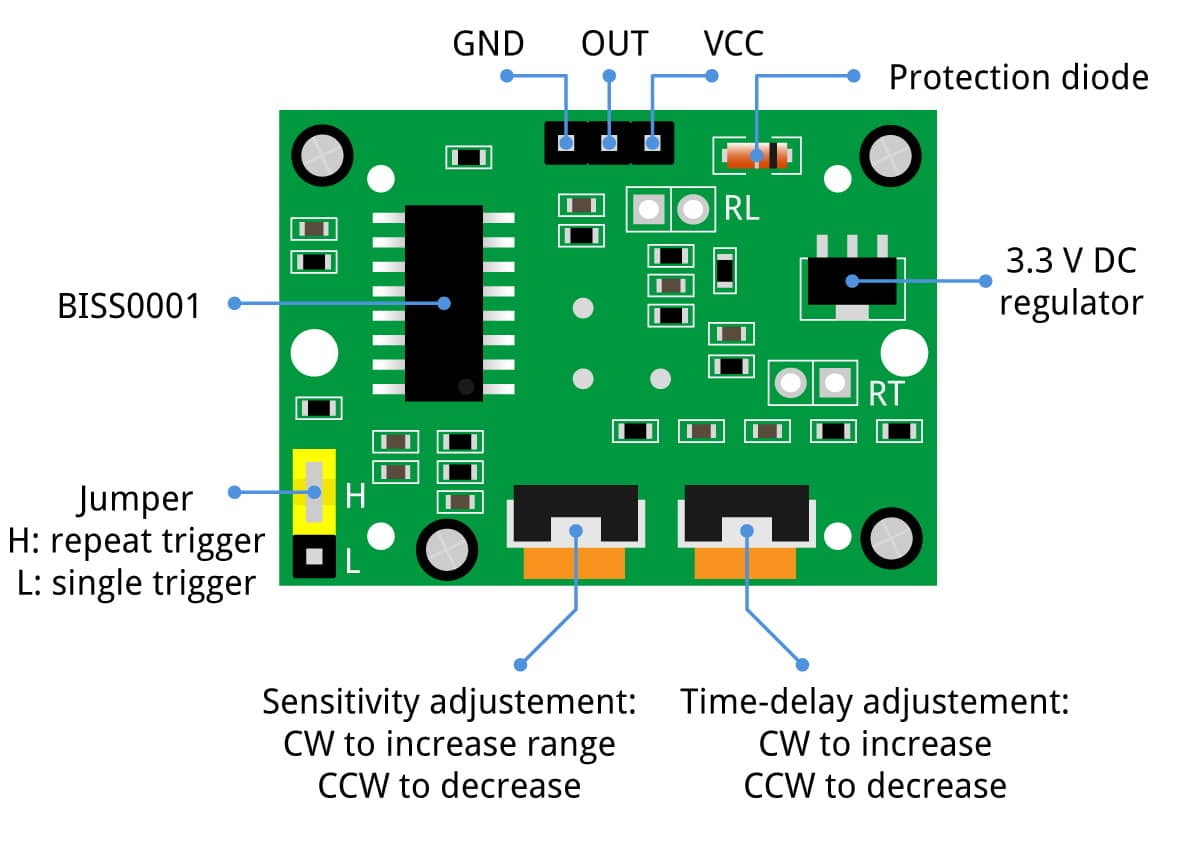
\includegraphics[width=0.5\textwidth]{images/hc-sr501_pinout.jpg}
	\caption{Pemetaan pin dan antarmuka modul PIR HC-SR501.}
	\label{fig:hc-sr501_pinout}
\end{figure}

\begin{table}[H]
    \centering
    \caption{Pemetaan pin antarmuka modul HC-SR501}
    \label{tab:hc_sr501_pin}
    \small
    \begin{tabularx}{\textwidth}{@{} p{3.2cm} p{2.2cm} X @{}}
        \toprule
        Pin (Modul Breakout) & Fungsi & Keterangan \\
        \midrule
        VCC  & $V_{CC}$ & Catu daya masukan ($5\text{ s.d. }12\,\text{V DC}$) \\
        OUT  & Sinyal & Keluaran logika digital biner ($3{,}3\,\text{V}$ HIGH / $0\,\text{V}$ LOW) \\
        GND  & GND & Referensi ground ($0\,\text{V}$) \\
        \bottomrule
    \end{tabularx}
\end{table}

Selain pin header antarmuka utama, modul HC-SR501 memiliki komponen penyesuaian parameter secara manual di atas papan PCB:

\begin{enumerate}
    \item \textbf{Antarmuka Potensiometer:}
    \begin{itemize}
        \item \textbf{Potensiometer Sensitivitas (\textit{Sensitivity Adjust}):} Terhubung ke sirkuit komparator internal BISS0001. Pemutaran searah jarum jam meningkatkan sensitivitas dan memperluas jarak deteksi hingga $\approx 7\,\text{meter}$, sedangkan pemutaran berlawanan arah jarum jam menurunkan jarak deteksi hingga $\approx 3\,\text{meter}$.
        \item \textbf{Potensiometer Waktu Tunda (\textit{Time Delay Adjust} / $T_x$):} Terhubung ke jaringan $RC$ pembuat pewaktu internal. Digunakan untuk mengatur durasi logika HIGH pada pin OUT saat gerakan terdeteksi dalam rentang $0{,}5\,\text{detik}$ hingga $\approx 200\,\text{detik}$.
    \end{itemize}

    \item \textbf{Antarmuka Konfigurasi Mode Pemicuan (\textit{Trigger Mode Jumper}):}
    \begin{itemize}
        \item \textbf{Mode L (\textit{Non-repeatable Trigger}):} Diaktifkan dengan menghubungkan \textit{jumper} ke pin posisi L. Pada mode ini, pewaktu $T_x$ dihitung murni dari awal gerakan, sehingga pin OUT akan beralih ke LOW setelah durasi $T_x$ usai meskipun objek masih terus bergerak.
        \item \textbf{Mode H (\textit{Repeatable Trigger}):} Diaktifkan dengan menghubungkan \textit{jumper} ke pin posisi H (mode bawaan pabrik). Pada mode ini, setiap gerakan baru akan mereset pewaktu $T_x$, sehingga pin OUT bertahan pada logika HIGH selama gerakan berlangsung hingga $T_x$ detik setelah gerakan fisik berhenti.
    \end{itemize}
\end{enumerate}

\subsubsection{Kebutuhan Catu Daya}
Modul HC-SR501 membutuhkan pasokan tegangan masukan eksternal dalam rentang $4{,}5\text{ s.d. }20\,\text{V DC}$ (umumnya dihubungkan ke rel $5\,\text{V DC}$ mikrokontroler). Papan pengembang modul telah mengintegrasikan IC regulator linier bertitik jatuh rendah (\textit{Low Dropout Voltage Regulator} / LDO) bertipe 7133-1 (atau setara HT7133) yang menurunkan tegangan masukan menjadi $3{,}3\,\text{V DC}$ ter-regulasi untuk mengoperasikan IC BISS0001 dan elemen sensor piroelektrik.

Arus konsumsi modul saat kondisi siaga (\textit{standby}) sangat rendah ($\approx 50\,\mu\text{A}$), menjadikannya sangat efisien untuk aplikasi sistem tertanam berbasis catu daya baterai. Karena sinyal keluaran logika biner pada pin OUT dikeluarkannya pada level $3{,}3\,\text{V}$ (HIGH), sinyal ini aman dihubungkan secara langsung (\textit{direct connection}) ke pin masukan digital mikrokontroler berlogika $3{,}3\,\text{V}$ (seperti ESP32 dan STM32) maupun mikrokontroler berlogika $5\,\text{V}$ (seperti Arduino Mega 2560 dan Uno) tanpa memerlukan Rangkaian Konverter Level Logika (\textit{Logic Level Shifter}).

% ---------------------------------------------------------------------
\subsubsection{Spesifikasi Penting dari Datasheet}
Rangkum parameter-parameter penting yang diambil langsung dari datasheet pabrikan resmi HC-SR501:

\begin{table}[H]
	\centering
	\caption{Spesifikasi penting modul HC-SR501}
	\label{tab:hc_sr501_spesifikasi}
	\small
	\begin{tabularx}{\textwidth}{@{}Xc@{}}
		\toprule
		Parameter                                             & Nilai             \\
		\midrule
		Tegangan kerja ($V_{CC}$)                             & $4{,}5 \text{ s.d. } 20$ $\text{V DC}$      \\
		Tegangan sinyal keluaran ($V_{\text{OUT}}$)           & $3{,}3$ (HIGH) / $0$ (LOW) $\text{V DC}$      \\
		Arus konsumsi (\textit{Standby})                      & $< 50$ $\mu\text{A}$      \\
		Jangkauan jarak deteksi                               & $3 \text{ s.d. } 7$ (Adjustable) $\text{m}$         \\
		Sudut jangkauan deteksi                               & $< 120$ $^\circ$ (Derajat) \\
		Waktu tunda keluaran ($T_x$)                          & $0{,}5 \text{ s.d. } 200$ (Adjustable) $\text{s}$         \\
		Waktu penguncian ulang (\textit{Blocking time} $T_i$) & $\approx 2{,}5$ $\text{s}$         \\
		Suhu operasional lingkungan                           & $-15 \text{ s.d. } +70$ $^\circ\text{C}$   \\
		Dimensi papan PCB                                     & $32 \times 24$ $\text{mm}$        \\
		\bottomrule
	\end{tabularx}
\end{table}

\subsubsection{Koneksi dengan Mikrokontroler dan Implementasi Kode}
Sensor HC-SR501 dihubungkan ke mikrokontroler Arduino Mega 2560 (ATmega2560) untuk mendeteksi pergerakan objek secara \textit{real-time}. Karena keluaran sensor berupa sinyal logika biner ($3{,}3\,\text{V}$ HIGH saat terdeteksi gerakan dan $0\,\text{V}$ LOW saat kondisi \textit{idle}), periferal utama yang dialokasikan pada mikrokontroler adalah pin \textbf{GPIO Digital Input} yang mendukung fungsi interupsi eksternal (\textit{External Interrupt}).

\paragraph{Rangkaian Skematik dan Simulasi}
Pengujian menggunakan simulator Wokwi. Konfigurasi koneksi antara modul HC-SR501 dan Arduino Mega 2560 diimplementasikan sebagai berikut:
\begin{itemize}
    \item \textbf{Koneksi Catu Daya:} Pin VCC modul dihubungkan ke rel daya $5\,\text{V}$ Arduino Mega 2560, dan pin GND dihubungkan ke pin ground mikrokontroller.
    \item \textbf{Koneksi Sinyal:} Pin OUT modul dihubungkan langsung ke pin digital $2$ Arduino Mega 2560 (yang mendukung jalur interupsi \texttt{INT0}). Tidak diperlukan pembagi tegangan (\textit{level shifter}) karena level tegangan $3{,}3\,\text{V}$ HIGH dari sensor sudah memenuhi ambang batas logika HIGH minimum pada ATmega2560 ($V_{IH} \approx 3{,}0\,\text{V}$).
\end{itemize}

\begin{figure}[htbp]
    \centering
    % Tangkapan layar simulasi Wokwi untuk antarmuka HC-SR501 dengan Arduino Mega 2560
    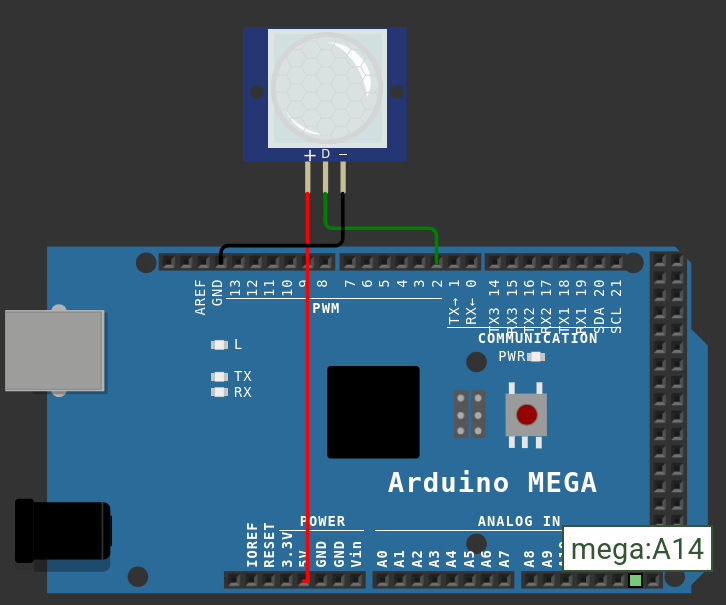
\includegraphics[width=0.70\textwidth]{images/hc-sr501_demo_wokwi.png}
    \caption{Rangkaian antarmuka modul HC-SR501 dengan Arduino Mega 2560 pada simulasi Wokwi.}
    \label{fig:hc_sr501_schematic}
\end{figure}

Rincian pemetaan koneksi fisik antara pin modul HC-SR501 dan fungsi periferal mikrokontroler ATmega2560 dirangkum pada Tabel~\ref{tab:hc_sr501_mcu_mapping}.
\begin{table}[H]
    \centering
    \caption{Pemetaan antarmuka modul HC-SR501 ke mikrokontroler Arduino Mega 2560}
    \label{tab:hc_sr501_mcu_mapping}
    \small
    \begin{tabularx}{\textwidth}{@{} p{3.5cm} p{3.8cm} X @{}}
        \toprule
        Kebutuhan Komponen & Fitur MCU & Alasan Pemilihan \& Fungsi \\
        \midrule
        Jalur Sinyal OUT & Pin GPIO Digital 2 (\texttt{INT0}) & Membaca tingkatan logika biner ($0\,\text{V}$ / $3{,}3\,\text{V}$) serta menyediakan jalur pemicuan interupsi eksternal \\
        Deteksi Peristiwa Gerakan & Interupsi Eksternal (\textit{Rising Edge}) & Mengeksekusi Rutin Pelayan Interupsi (\textit{Interrupt Service Routine} / ISR) secara asinkron saat sinyal beralih ke logika HIGH \\
        Catu Daya Operasional & Rel $5\,\text{V}$ \& GND MCU & Memasok daya operasional ter-regulasi untuk sirkuit internal BISS0001 dan elemen piroelektrik \\
        \bottomrule
    \end{tabularx}
\end{table}

\paragraph{Kode Demo Pengujian}
Berikut adalah implementasi program pengujian antarmuka HC-SR501 pada Arduino Mega 2560 menggunakan pendekatan \textit{Interrupt Service Routine} (ISR) berbasis interupsi eksternal:

\begin{lstlisting}[language=C++, caption={Kode program pengujian sensor HC-SR501 berbasis interupsi pada Arduino Mega 2560}, label={lst:hc_sr501_code}]
#define PIR_PIN 2
volatile bool motionDetected = false;

void pirISR() {
  motionDetected = true;
}

void setup() {
  Serial.begin(9600);
  Serial.println(F("Inisialisasi Pengujian Sensor HC-SR501..."));
  pinMode(PIR_PIN, INPUT);
  attachInterrupt(digitalPinToInterrupt(PIR_PIN), pirISR, RISING);
}

void loop() {
  if (motionDetected) {
    Serial.println(F("[TERDETEKSI] Pergerakan objek termal terdeteksi!"));
    motionDetected = false;
  } else {
    Serial.println(F("[STANBY] Tidak ada gerakan (Kondisi Aman)"));
  }

  delay(1000);
}
\end{lstlisting}

\paragraph{Gambaran Hasil Pembacaan}
Setelah skrip dijalankan di simulator Wokwi, luaran pembacaan data pada \textit{Serial Monitor} saat pengujian simulasi gerakan akan tampil seperti contoh berikut:

\begin{verbatim}
Inisialisasi Pengujian Sensor HC-SR501...
[STANBY] Tidak ada gerakan (Kondisi Aman)
[TERDETEKSI] Pergerakan objek termal terdeteksi!
[STANBY] Tidak ada gerakan (Kondisi Aman)
\end{verbatim}
